%%%%%%%%%%%%%%%%%%%%%%%%%%%%%%%%%%%%%%%%%%%%%%%%%%%%%%%
%                File: OpEx_temp.tex                  %
%                  Date: Sept. 2, 2009                %
%                                                     %
%           LaTeX template file for use with          %
%           OSA's journal Optics Express              %
%                                                     %
%  send comments to Jennifer Mayfield, jmayfi@osa.org %
%                                                     %
% This file requires style file, opex3.sty, under     %
%              the LaTeX article class                %
%                                                     %
%   \documentclass[10pt,letterpaper]{article}         %
%   \usepackage{opex3}                                %
%                                                     %
% Note that our online submission system does not     %
% currently process PDFLaTeX; if PDFLaTeX must be     %
% used, pls. contact OpEx staff, and we will process  %
% manually                                            %
%                                                     %
%                                                     %
%       (c) 2009 Optical Society of America           %
%%%%%%%%%%%%%%%%%%%%%%%%%%%%%%%%%%%%%%%%%%%%%%%%%%%%%%%

%%%%%%%%%%%%%%%%%%%%%%% preamble %%%%%%%%%%%%%%%%%%%%%%%%%%%
\documentclass[10pt,letterpaper]{article}
\usepackage{{../lib/opex3}}
%\usepackage{{../lib/penarandaY}}
\graphicspath{{../Pictures/}}
\usepackage{caption}
\usepackage{subcaption}
\usepackage{amsmath} % Required for equation and aligned environments
\usepackage{hyperref}
\RequirePackage{numprint}

%\usepackage{ae} %%for Computer Modern fonts

%%%%%%%%%%%%%%%%%%%%%%% begin %%%%%%%%%%%%%%%%%%%%%%%%%%%%%%
\begin{document}

%%%%%%%%%%%%%%%%%% title page information %%%%%%%%%%%%%%%%%%
\title{Chromatic Objective Design for Extended Depth of Focus \textit{(EDOF)}}

\author{M. Gostiaux Gabriel, M. Yohan Penaranda}

\address{M. Gabriel Gostiaux, Master of Science student, Institute of Optics, \\ Palaiseau, 91 120, France}

\email{gabriel.gostiaux@institutoptique.fr} %% email address is required

%\homepage{https://github.com/GabrielGst?tab=repositories} %% author's URL, if desired

%%%%%%%%%%%%%%%%%%% abstract and OCIS codes %%%%%%%%%%%%%%%%
%% [use \begin{abstract*}...\end{abstract*} if exempt from copyright]

\begin{abstract*}
This study introduces basic concepts of co-design to optimize parameters of a chromatic imaging system dedicaetd to EDOF using high-frequency transfer algorithm to enhance RGB image resolution.
\linebreak

\textbf{Keywords:} EDOF, high frequency transfer, chromatic imaging system.
\linebreak

\end{abstract*}

\ocis{(000.0000) General.} % REPLACE WITH CORRECT OCIS CODES FOR YOUR ARTICLE

%%%%%%%%%%%%%%%%%%%%%%% References %%%%%%%%%%%%%%%%%%%%%%%%%
\begin{thebibliography}{99}

%\bibitem{labwork} F. Goudail, D. Bloch, O. Leveque, ``FED labworks and projects,'' IOGS {\bf lab 3-4-5,} (2024)
\bibitem{trouve} P. TROUVE, ``Co-conception pourr la mesure 3D,'' IOGS, 11--25 (2024).
\bibitem{TNT+08} C.L. Tisse, H.P. Nguyen, R. Tessières, M. Pyanet, and F. Guichard. ``Extended
depth-of-field (EDoF) using sharpness transport across colour channels,'' In
Society of Photo-Optical Instrumentation Engineers (SPIE) Conference Series, {\bf volume 7061, page 4} (2008).

\end{thebibliography}

%%%%%%%%%%%%%%%%%%%%%%%%%%  body  %%%%%%%%%%%%%%%%%%%%%%%%%%
\section{Introduction}
One of the many objectives of co-design is to simulate optical designs in order to optimize costs through reducing the number of elements of the optical chain of a system. It is also possible to replace costly elements with hybrid ones, integrating signal and image processing in the system.

Here, we will focus on two methods for extended depth of focus. The first section deals with the design of a EDOF algorithm which uses high frenquency transfer, applied to real images acquired with a chromatic imaging system. The second section will dive into the modelling of such a chromatic system. We will see how optimizing the curvature radius and the focus, can be monitored by the criteria of maximizing the range within which at least one of the channels is resolved. This is actually equivalent to maximizeing the union of the depth of focus of the three RGB channels of a chromatic camera within a range of interest.

\section{High Frequency Transfer}
This study introduces basic concepts of co-design to optimize parameters of a chromatic imaging system dedicated to EDOF using high-frequency transfer algorithm to enhance RGB image resolution. The method, presented in \cite{TNT+08}consist in adding to each channel the high frequencies of all the other channels, weighted by the resolution level of each channel. This can be expressed as :

\begin{equation}\label{eqn:HFT}
    y_{c}^{EDOF} = y_{c}^{init} + \alpha . HF_R + \beta . HF_G + \gamma . HF_B
\end{equation}

\pagebreak

We will see how the resolution can be improved regarding the depth of focus, even after the acquisition of the image. One can see the original picture on fig. \ref{sub@fig:origin} and the enhanced picture on fig. \ref{sub@fig:edof} .

\begin{figure}[h]
    \centering
    \subfloat[Original picture]{
        \centering
        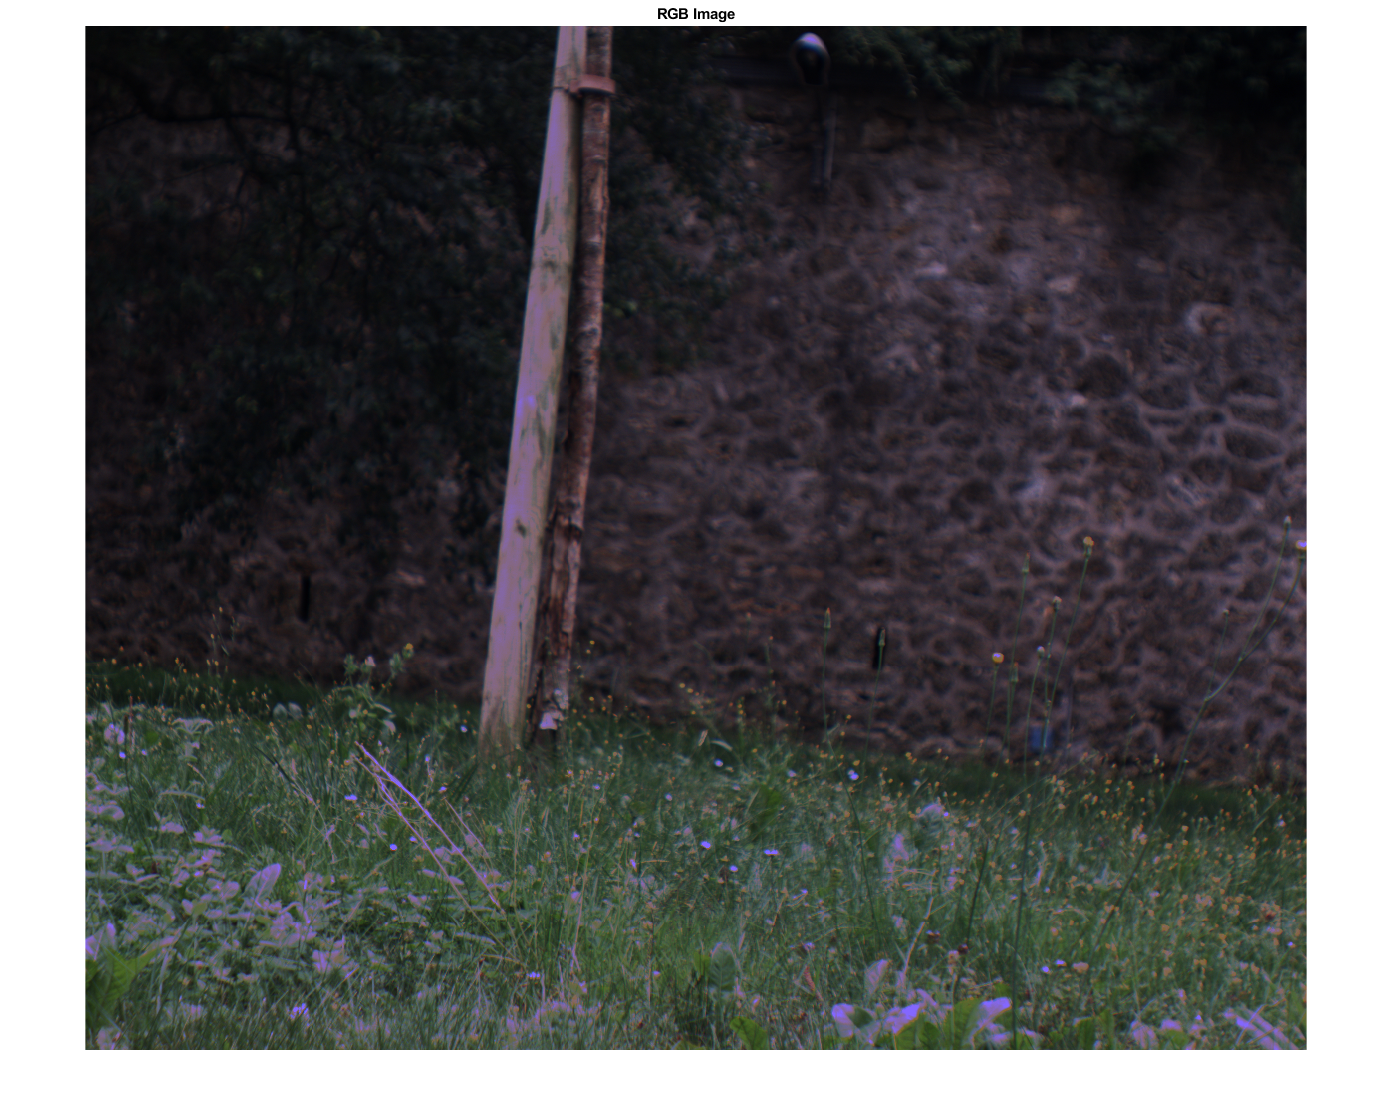
\includegraphics[width=0.3\textwidth]{Original picture.png}
        \label{fig:origin}
    }
	\subfloat[Optimized pîcture]{
		\centering
        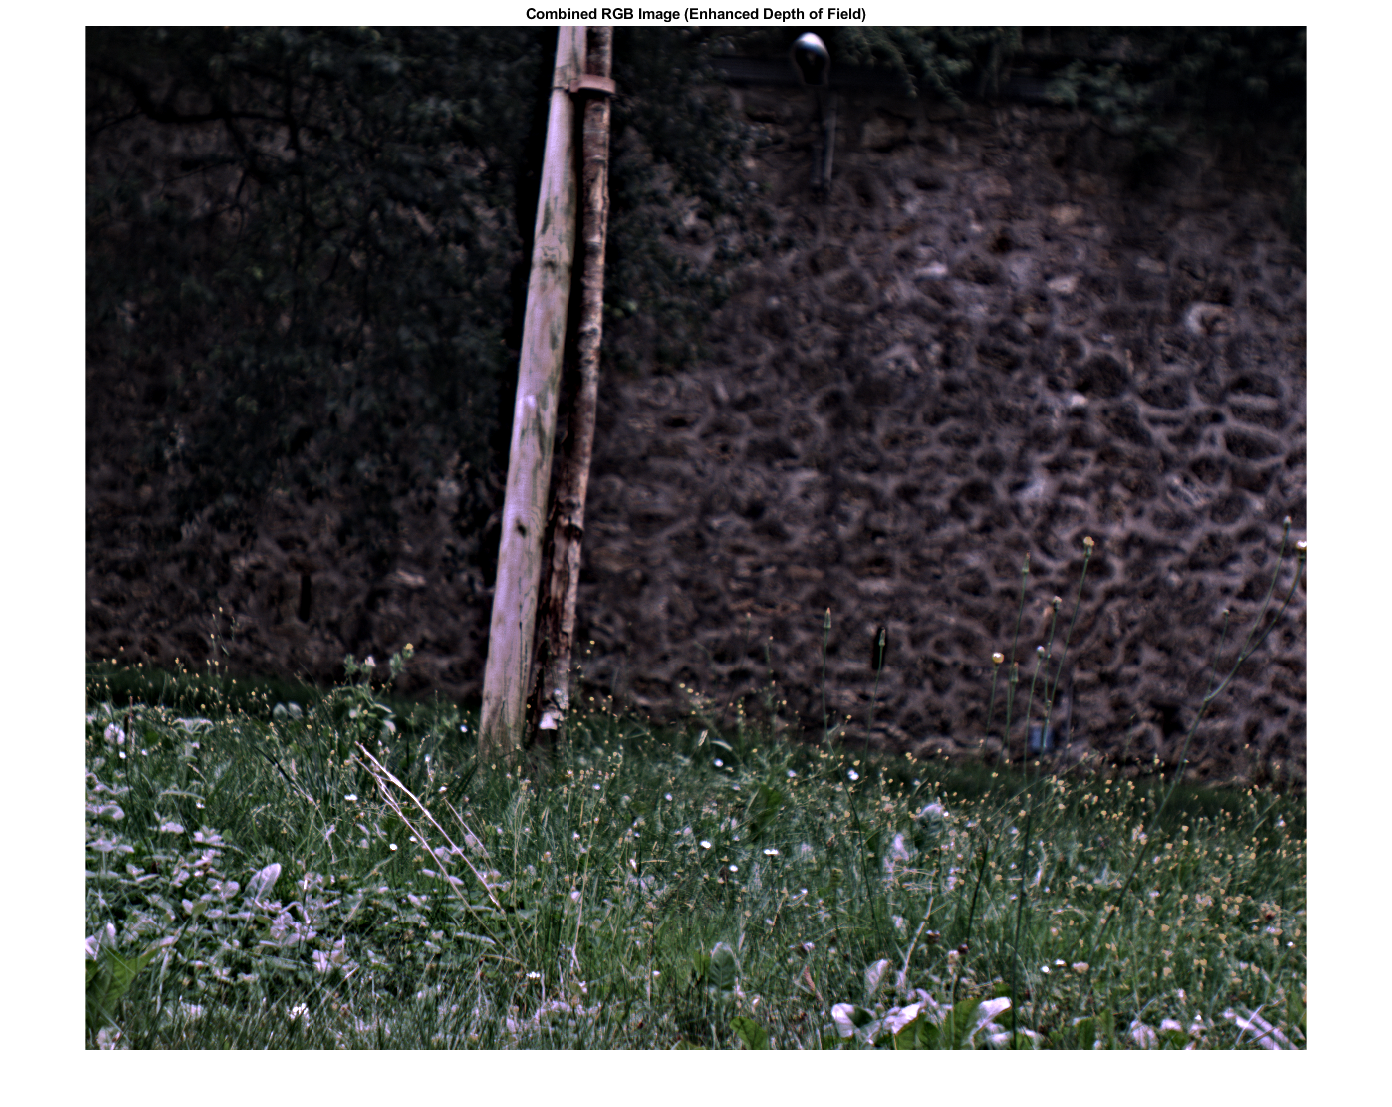
\includegraphics[width=0.3\textwidth]{Final EDOF.png}
        \label{fig:edof}
    }
	\caption{High Frequency Transfer}
\end{figure}

We will talk about the multiple improvements in resolution at the end of the section, and focus on presenting the method that led to the EDOF picture.

\subsection*{Coefficient computation}
We start by separating the three R, G, B channels constituying the image, and we look at them separately : one can figure that the resolution is best for the red channel, and worst for the blue channel. This is caused by chromatic dispersion of glass in the lenses of the optical imaging system.

\begin{figure}[h]
	\centering
	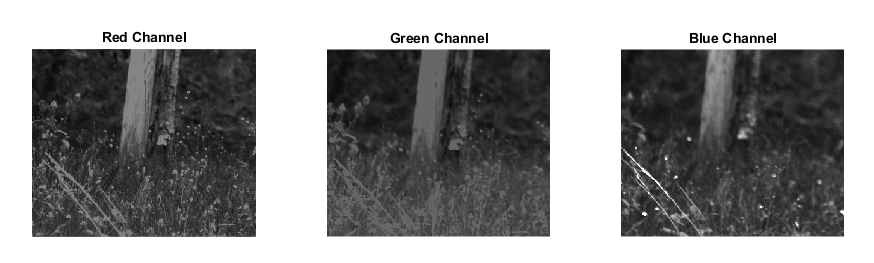
\includegraphics[scale=0.45]{Channels Original and Blured DOF.png}
	\caption{Blured blue and green channels}
	\label{fig:blured-channels}
\end{figure}

Let us now compute the coefficients $\alpha,\beta,\gamma$ thanks to the expression of the gradients computed on the different channels, according to the formula:

$$
\begin{aligned}
\alpha & =\frac{\left\|\Delta_{y_R}\right\|^2}{\left\|\Delta_{y_R}\right\|^2+\left\|\Delta_{y_V}\right\|^2+\left\|\Delta_{y_B}\right\|^2} \\ 
\beta & =\frac{\left\|\Delta_{y_V}\right\|^2}{\left\|\Delta_{y_R}\right\|^2+\left\|\Delta_{y_V}\right\|^2+\left\|\Delta_{y_B}\right\|^2} \\ 
\gamma & =\frac{\left\|\Delta_{y_B}\right\|^2}{\left\|\Delta_{y_R}\right\|^2+\left\|\Delta_{y_V}\right\|^2+\left\|\Delta_{y_B}\right\|^2}\end{aligned}
$$

We apply a mean filter in order to smooth those gradients and work within the surroundings of the details contained in the image.

\begin{figure}[h]
    \centering
    \subfloat[Gradients of each channels]{
        \centering
        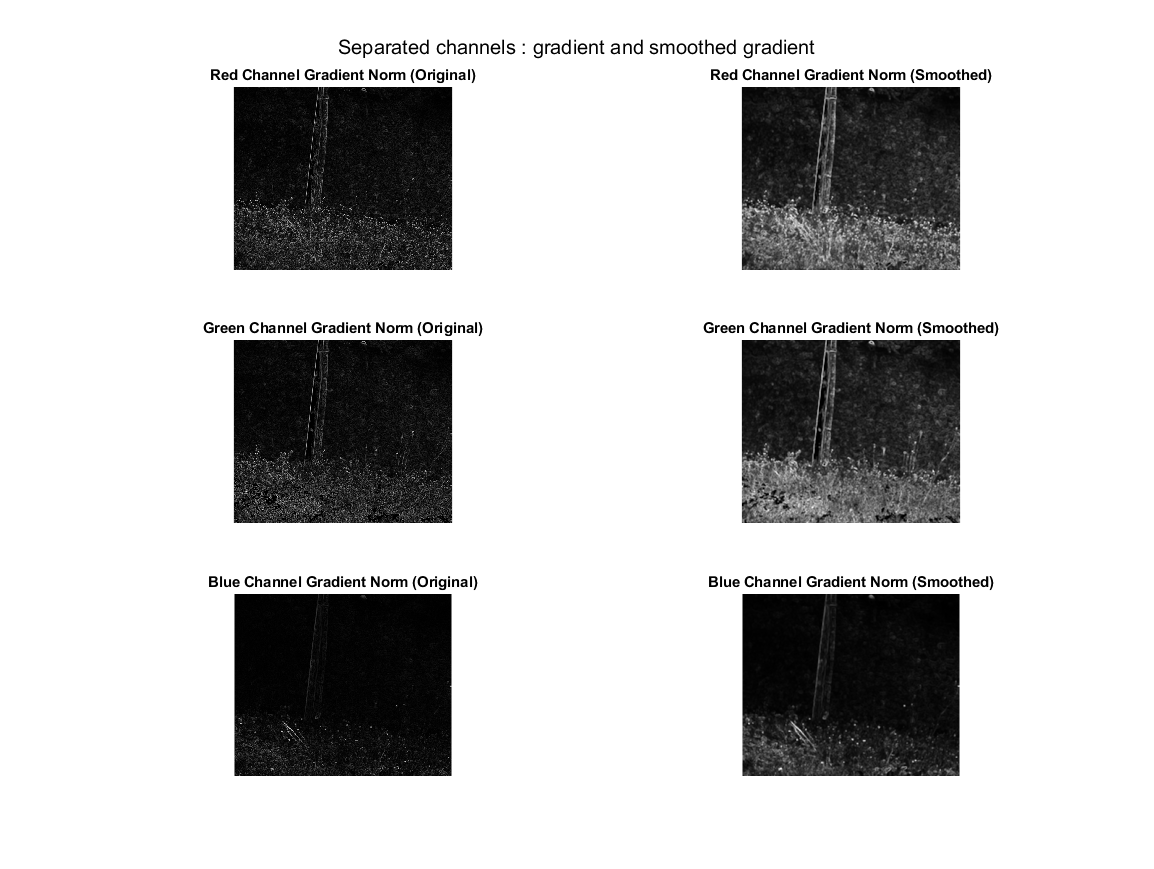
\includegraphics[width=0.45\textwidth]{Channels Gradient Norms (orig vs smothed).png}
        \label{fig:gradients}
    }
	\subfloat[High frequency channels]{
		\centering
        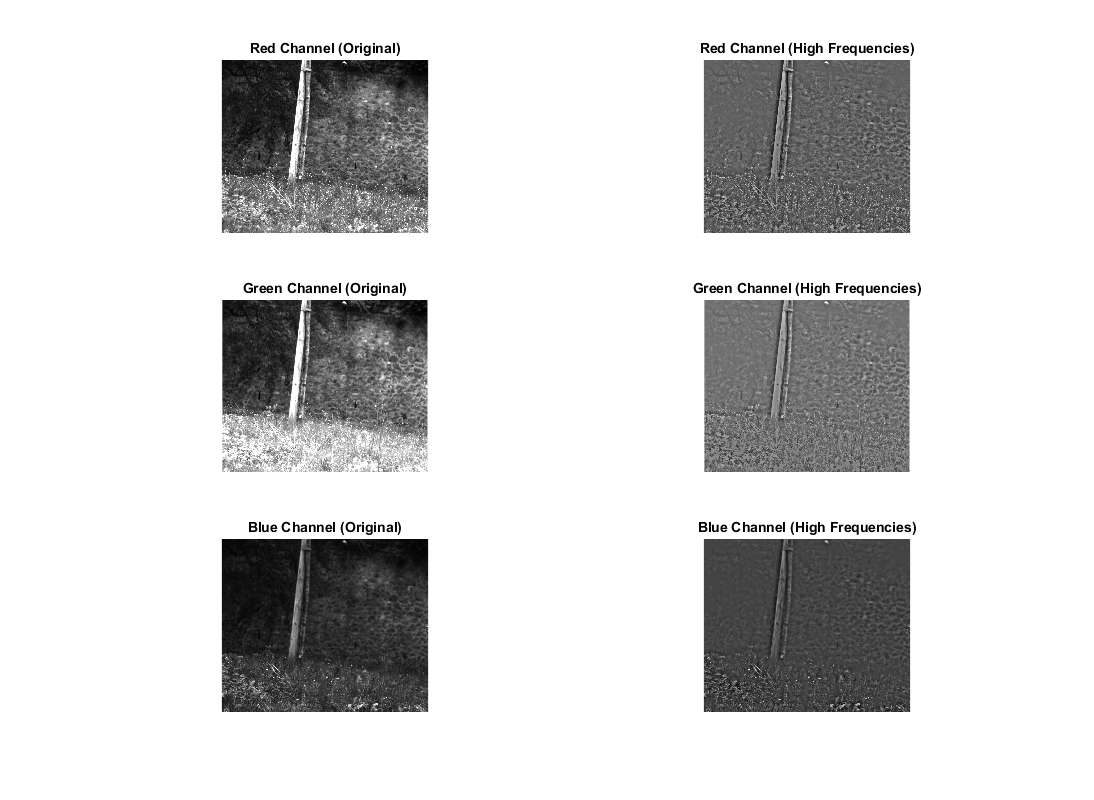
\includegraphics[width=0.45\textwidth]{Channels High Freq.png}
        \label{fig:hfc}
    }
	\caption{High Frequency Transfer}
\end{figure}

Let us then extract the high frequency components of each channels, in order to apply the equation \ref{eqn:HFT} and compute the resolved channels. In this purpose, we compute the convolution of the channels with a large PSF ($s = 50$) to obtain the low frequencies.  We then substract them from the initial channel to obtain the remaining high frequencies, as can be seen on fig. \ref{fig:hfc} .

We thus obtain three corrected channels, as can be seein on fig. \ref{fig:edof-channels} .

\begin{figure}[h]
    \centering
    \subfloat[EDOF channels]{
        \centering
        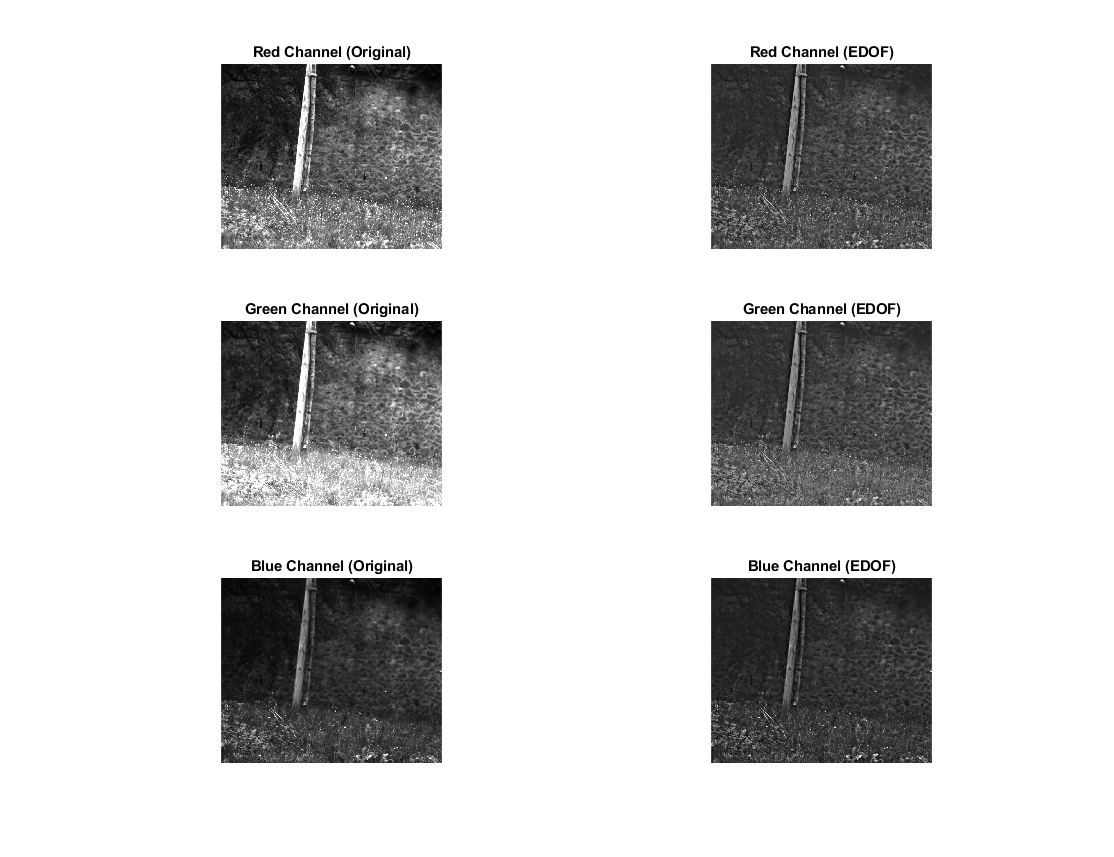
\includegraphics[width=0.45\textwidth]{EDOF channels.png}
        \label{fig:edof-channels}
    }
	\subfloat[EDOF channels (zoomed)]{
		\centering
        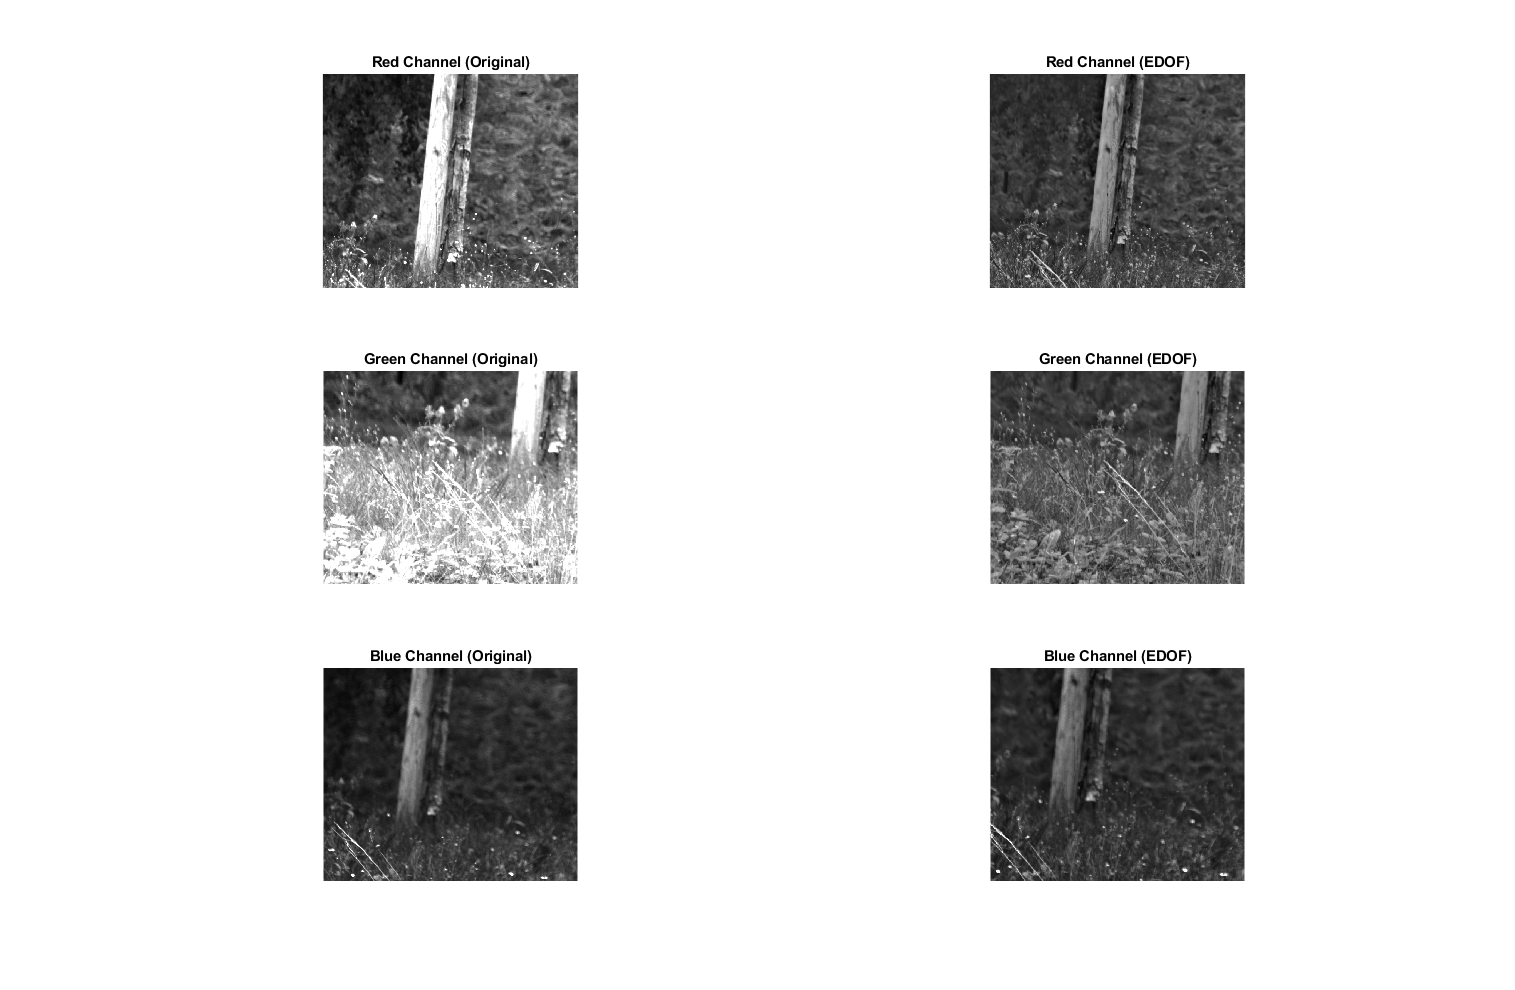
\includegraphics[width=0.53\textwidth]{EDOF channels zoomed.png}
        \label{fig:edof-channels-zoomed}
    }
	\caption{High Frequency Transfer}
\end{figure}

\subsection*{Results and discussion}
Applying the high frequency transfer algorithm to an image helps improving chromatic defocus, but it also seems to flatten the image by reducing saturation (mostly on the green channel).

In regard of fig. \ref{fig:cutoff} on which are presented the EDOF pictures according to the cutoff frequency of the lowpass filter (which parameter is the size of the PSF), one can see that the effect of the HF transfer is to emphasize the details of the high frequencies which have not been filtered, thus degrading contrast of highly detailed zones over the image (such as the bark of the tree). Thus, one could define a mid-range threshold that would lead to a resolution trade-off between highly-detailed and poorly-detailed zones. One could also apply a different threshold according to a spatial parameter representing the level of detail of one zone in the image.

\begin{figure}[h]
	\centering
	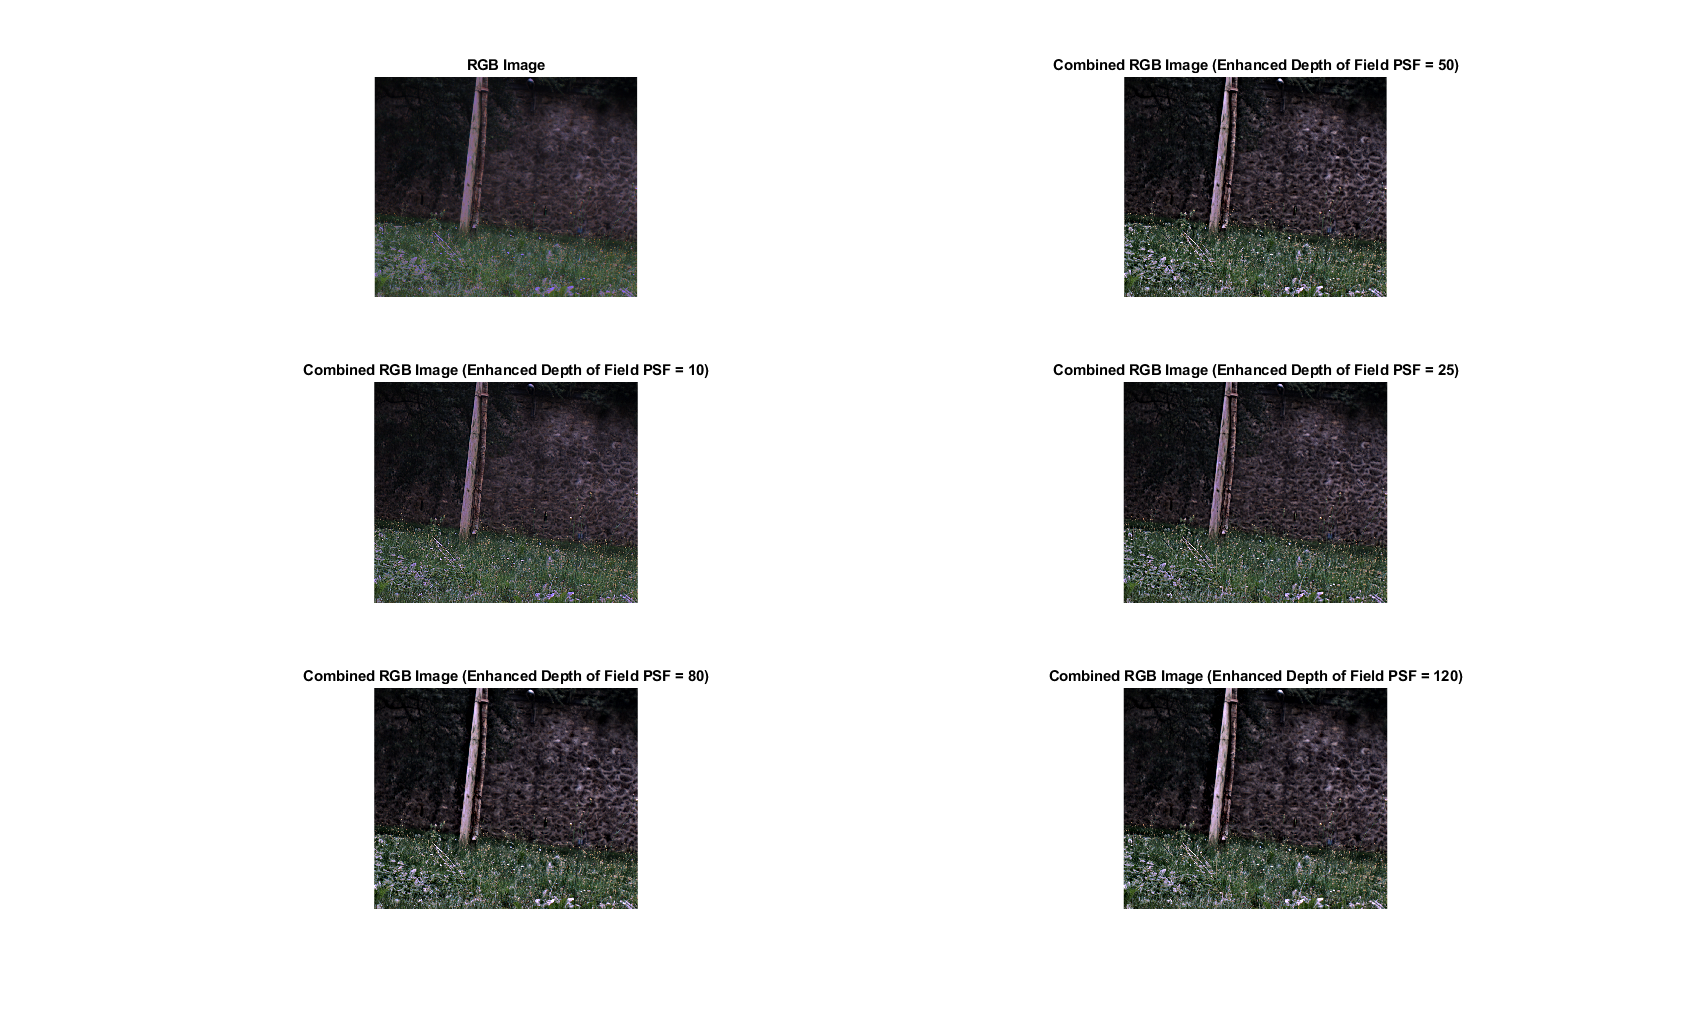
\includegraphics[scale=0.25]{PSF variating EDOF RGB.png}
	\caption{EDOF, variating frequency cutoff}
	\label{fig:cutoff}
\end{figure}





\section{Chromatic Imaging Design}
\paragraph{Position capteur}
$$\frac{1}{x'_0} - \frac{1}{x_0} = \frac{1}{f'}$$
$$x'_0=\frac{1}{\frac{1}{f'} + \frac{1}{x_0}} = \numprint[mm]{25.3}$$

\paragraph{Profondeur de champ}
$$x_{min} = \frac{x'0}{1-\frac{x'0}{f'} + \frac{t_{px}}{D}} = \numprint[m]{-2.0925}$$
$$x_{max} = \frac{x'0}{1-\frac{x'0}{f'} - \frac{t_{px}}{D}} = \numprint[m]{-1.9152}$$
Donc profondeur de champ $\numprint[m]{0.1773}$
\listoffigures

\end{document} 
